\documentclass{bio}
%\documentclass[oupdraft]{bio}
\usepackage[colorlinks=true, urlcolor=citecolor, linkcolor=citecolor, citecolor=citecolor]{hyperref}
\usepackage[utf8]{inputenc}
\usepackage[english]{babel}

% Add history information for the article if required
%\history{}


%% NOTES TO SELF:
% Cite using:
%    \citet{...}  in text
%    \citealp{...}   within parantheses
%
% Temporary notifications and reminders:
%    \COMMENT{text}{comment to text}
%    \NB{comment (as separate paragraph)}
%    \NOTE{comment inside paragraph}
%    \CITE{missing/unspecified citation}
\usepackage{color}
\definecolor{NBcol}{rgb}{0.7,0,1}
\definecolor{CITEcol}{rgb}{1,0,0.7}
\definecolor{COMMENTcol}{rgb}{0.7,0.2,0}
\newcommand\COMMENT[2]{\textcolor{COMMENTcol}{#1}\NOTE{#2}}
\newcommand\NB[1]{\textcolor{NBcol}{\textit{#1}}}
\newcommand\NOTE[1]{\NB{[#1]}}
\newcommand\CITE[1]{\textcolor{CITEcol}{[#1]}}


\begin{document}

\footnotetext{\color{blue}Manuscript version \today.}

% Title of paper
\title{Methods that remove batch effects while retaining group differences may lead
to exaggerated confidence in downstream analyses
}

% List of authors, with corresponding author marked by asterisk
\author{VEGARD NYGAARD, EINAR ANDREAS RØDLAND\\[4pt]
% Author addresses
\textit{Department of Tumor Biology,
Institute for Cancer Research,
Oslo University Hospital HF - Radiumhospitalet,
Montebello,
0310 Oslo,
Norway}
\\[8pt]
EIVIND HOVIG$^\ast$\\[4pt]
% Author addresses
\textit{Department of Tumor Biology,
Institute for Cancer Research,
Oslo University Hospital HF - Radiumhospitalet,
Montebello,
0310 Oslo,
Norway}
\\[2pt]
\textit{\NOTE{Andre adresser}}
\\[2pt]
% E-mail address for correspondence
{ehovig@ifi.uio.no}}

% Running headers of paper:
\markboth%
% First field is the short list of authors
{V. Nygaard, E. A. Rødland, E. Hovig}
% Second field is the short title of the paper
{Exaggerated effects after batch correction}


\maketitle


% Add a footnote for the corresponding author if one has been
% identified in the author list
\footnotetext{To whom correspondence should be addressed.}

\begin{abstract}
{Removal of, or adjustment for, batch effects or centre differences is generally required when such effects are present in data. In particular, when preparing microarray gene expression data from multiple cohorts, array platforms, or batches for later analyses, batch effects can have confounding effects. Many methods and tools exist for this purpose. One method, ComBat which is part of the R package sva, is particularly popular due to its ability to remove batch differences even when batches are small and heterogeneous. It also has the option of preserving the difference between study groups, estimated from a two-way ANOVA model, to avoid conflating batch effects and group differences during batch adjustments. Unfortunately, this frequently used and recommended approach may systematically induce incorrect group differences in downstream analyses when groups are distributed between the batches in an unbalanced manner. The scientific community seems to be largely unaware of this problem, which most likely has contributed to false discoveries being presented in the published literature.
}
\end{abstract}


\section{Introduction}\label{intro}

Extraneous variables, if left unaccounted for, have the potential to lead an investigator into drawing wrong conclusions. A common example is ``batch effects'' caused by reagents, microarray chips, and other equipment made in batches, which often have systematic effects on the measurements. A similar example is ``centre effects'' when samples or data come from multiple sources. See \citet{Luo2010} for more examples.

For a typical experiment comparing differences between study groups, the presence of batch effects will decrease the statistical power since it adds variation to the data. If the batch--group design is unbalanced, i.e if the study groups are not equally represented in all batches, batch effects may also act as a confounder and induce false differences between groups (\citealp{Leek2010}).

The standard way to handle an extraneous variable is to include it in the statistical model employed in the inquiry. However, many analysis tools for high throughput data do not cater for this option, and when available it could still be outside the competence of the investigator. Therefore, an alternative two step procedure has emerged. First the batch effects are estimated and removed, creating a ``batch effect free'' data set. Then, the statistical analyses are performed on the adjusted data without further consideration of batch effects. This appealing compartmentalization is also convenient for practical purposes, for example when data-processing and statistical analyses are performed by different personnel. Unfortunately, as we demonstrate in this paper, when the batch--group design is unbalanced, this approach may be unreliable.

A simple removal of batch effects can be achieved by subtracting the mean of the measurements in one batch from all measurements in that batch, i.e mean adjustment or one-way ANOVA adjustment as implemented in the method \texttt{pamr.batchadjust} from the \texttt{pamr} package in R. When the batch--group design is balanced, mean-adjustment will remove most, but not necessarily all, variance attributed to batch and leave the between group variance, thus increasing the statistical power. However, when the batch--group design is unbalanced, batch differences will in part be influenced by group differences, and thus batch correction will reduce group differences and thereby reduce the statistical power. In very uneven group--batch designs with multiple groups, spurious group differences may even be induced in this way. Figure~\ref{fig:boxplots} illustrates both these effects.

To mitigate the above problems, one may simultaneously estimate batch effects and group differences, e.g. using a two-way ANOVA, and only remove the batch differences from the data. Effectively, group differences are estimated based on within batch comparisons, and applied to the batch adjusted data. In a balanced group--batch design, estimates of group differences and batch effects are independent, and this approach becomes identical to the above described zero-centering per batch. However, if the group--batch design is heavily unbalanced, estimation of group differences and batch effects are interdependent, and when applying the estimated group differences across the entire data set, the uncertainties of these estimates are ignored. Subsequent analyses will then systematically underestimate the statistical uncertainties and exaggerate the confidence of group differences. Figure~\ref{fig:boxplots} illustrates how statistical uncertainties are deflated by this batch adjustment method by comparing them to the uncertainties from the original ANOVA.

The ComBat method described in \citet{Johnson2007}, and included in the \texttt{sva} package (\citealp{Leek2012}), can use either of the two above described approaches to estimate batch differences. In addition, it uses an empirical Bayes approach to avoid over-correction for batch effects, which is critical for small batches. Increasingly, the inclusion of group difference as a covariate when removing batch effects has been recommended, both in the \texttt{sva} tutorial and user fora, and ComBat has thus help popularise this approach. Based on actual use of ComBat by the authors and others, ourselves included, we suspect thus adjusted data are commonly treated as ``batch effect free'' in subsequent analyses. And as a consequence, confidence in group effects has been overestimated and false results reported.

Statisticians would most likely take extra precautions should the sample or batch sizes be very small. However, the effects of batch adjustment using two-way ANOVA or ComBat on unbalanced data sets remain even as sample and batch sizes increase. For example, group comparisons using one-way ANOVA on the batch adjusted data will essentially result in $F$ statistics that are inflated by a fixed factor which depends on the unevenness of the design rather than the size of the sample or batches. The effect of this may be further exacerbated by running these analyses a large number of times, e.g. on thousands of genes, and use false discovery rate to determine significant cases: an approach that is particularly sensitive to inflated false positive rates.


\section{Methods for batch effect correction}

\subsection{Model for data with batch effects}

We will base our discussion on a simple model for data with batch effects:
\begin{equation}
Y_{ijr}=\alpha+\beta_j+\gamma_i+\epsilon_{ijr}
\end{equation}
where $i=1,\ldots,m$ are the different batches, $j=1,\ldots,M$ are different study groups that we wish to compare, and $\epsilon_{ijr}\sim N(0,\sigma^2)$ are the error terms for samples $r=1,\ldots,n_{ij}$ within batch $i$ and group $j$.

When combining data from more diverse data sources, e.g. microarray data from different platforms, a more general model is required. One such model, used by \citet{Johnson2007}, is
\begin{equation}
Y_{ijgr}=\alpha_g+X_r\beta_{g}+\gamma_{ig}+\delta_{ig}\epsilon_{ijgr}
\end{equation}
where $g=1,\ldots,G$ are different measurements, e.g. genes, performed for each sample, and $X$ is the design matrix which in our case will indicate the study group. This permits independent rescaling of data from different batches. In addition, \citet{Johnson2007} uses an empirical Bayes approach to estimate $\gamma_{ig}$ and $\delta_{ig}$ to stabilise estimates, which is critical for use with small batches.

For simplicity, we consider the case with a single gene and constant scale, i.e. $\delta_{ig}=1$. Empirical Bayes will tend to shrink the estimates of  $\gamma_{ig}$, and thus the amount of batch adjustment, in cases where batch effects are small or cannot be accurately estimated, e.g. for small batches. However, in cases with large batches or substantial batch effects, it should differ little from the two-way ANOVA approach. We will therefore explain the problem in the simpler case where no empirical Bayes is applied, and later demonstrate that it also affects the ComBat approach.

\subsection{Standard batch correction methods}

A common ambition of batch effect adjustments is to remove batch differences in such a way that downstream analyses of the adjusted data may be done without further corrections for batches. We illustrate this using Figure~\ref{fig:boxplots}, where the first frame contains the ``true'' values with no batch differences, and the remaining frames show values with various levels of batch effects and batch effect corrections.

The most common method for removing batch effects is to zero-centre each batch:
\begin{equation}
\Delta\widetilde Y_{ijr}=Y_{ijr}-\bar{Y}_{i}
\quad\text{where}\quad
\bar{Y}_i=\frac{\sum_{j=1}^M\sum_{r=1}^{n_{ij}} Y_{ijr}}{\sum_{j=1}^M n_{ij}}.
\end{equation}
An alternative is to centre each batch to the common average by adding the average value $\bar{Y}$ across the entire data set: i.e. $\widetilde Y_{ijr}=\Delta\widetilde Y_{ijr}+\bar{Y}$. When comparing groups, the common value $\bar{Y}$ has no effect, and so this is equilvalent to zero-centring each batch. If the groups are unevenly represented in the different batches, the batch average $\bar{Y}_i$ will tend to capture, through $\bar\beta_i$, group differences as well as batch effects:
\begin{equation}
\Delta\widetilde{Y}_{ijr}=\beta_j-\bar{\beta}_i+\epsilon_{ijr}-\bar{\epsilon}_i
\quad\text{where}\quad
\bar{\beta}_i=\frac{\sum_{j=1}^M n_{ij}\beta_j}{\sum_{j=1}^M n_{ij}},\;
\bar{\epsilon}_i=\frac{\sum_{j=1}^M\sum_{r=1}^{n_{ij}} \epsilon_{ijr}}{\sum_{j=1}^M n_{ij}}.
\end{equation}
Thus, batch centering will tend to reduce group differences in an unbalanced design, and reduce the power of downstream analyses. By reducing the differences between some groups, i.e. those found together in the same batches, it may also induce false differences between other groups, as is demonstrated in Figure~\ref{fig:boxplots}.

Removing batch effects while retaining group differences can be done through a two-way ANOVA in which group effects, $\beta_j$, and batch effects, $\gamma_i$, are estimated simultaneously. Batch adjusted values may then be obtained by subtracting the estimated batch effects, $\hat\gamma_i$:
\begin{equation}
\widetilde Y_{ijr}=Y_{ijr}-\hat\gamma_i=\alpha+\beta_j+(\gamma_i-\hat\gamma_i)+\epsilon_{ijr}.
\end{equation}
This will yield batch adjusted values where any systematic bias induced by the batch differences has been removed, while the group differences are retained.

The estimation error $\hat\gamma_i-\gamma_i$ affects all values within the same batch in the same manner. Thus, while the aim is to remove spurious dependencies within batches, it may also induce new dependencies. The batch effect estimation errors will influence group effects in proportion to how well the group is represented in each batch:
\begin{equation}
\widetilde{Y}_{\textrm{-}j}
=\frac{\sum_{i=1}^m\sum_{r=1}^{n_{ij}}\widetilde{Y}_{ijr}}{n_{\textrm{-}j}}
=\alpha+\beta_j+\bar{\epsilon}_{\textrm{-}j}
  -\sum_{i=1}^m \frac{n_{ij}}{n_{\textrm{-}j}}(\hat{\gamma}_i-\gamma_i),
\quad
n_{\textrm{-}j}=\sum_{i=1}^m n_{ij}.
\end{equation}
In a balanced group--batch design, the effect is the same all groups and thus does not influence group comparisons. In an unbalanced design, however, the estimation errors $\hat\gamma_i-\gamma_i$ will induce systematic differences between groups which, when ignored in downstream analyses, may lead to over-confidence in estimated group differences. In Figure~\ref{fig:boxplots}, the effect of batch correction using group as covariate is shown with confidence intervals of the corrected data. For comparison, least square means estimates (R package \texttt{lsmeans}) are used to illustrate more appropriate confidence intervals that incorporate the uncertainties of the estimation errors.


\section{Results}

\subsection{A simple sanity check}

The undesired consequences of preserving group effects when correcting for batch effect is readily illustrated with a sanity check using random numbers. The documentation accompanying the \texttt{sva} library has a runnable example demonstrating how to adjust a data set with ComBat followed by an F-test. Replacing the real data with random numbers from a standard normal distribution (mean=0, sd=1), but otherwise following the instructions, will generate the p-value distribution shown in Figure~\ref{fig:sanity}.

As can be seen from the QQ plot, the main effect of the procedure is to inflate the F-statistic by a factor. The size of this factor depends on how unbalanced the group--batch design is rather than on the sample size in itself. Thus, increasing the sample size will not reduce the problem.

If the number of samples is increased and there are no actual batch effects present, the empirical Bayes estimates used by ComBat will shrink the batch effect estimates and thus moderate the batch adjustments. However, if batch differences are added which are not constant across all genes, the problem remains even as the samples size increases.

\subsection{Explanation for the simple two-group comparison}
\label{sec:twogroups}

To explain more clearly what is happening, and quantify the size of the problem, we may consider the simple case of estimating the difference $\Delta\beta=\beta_A-\beta_B$ between two groups, $A$ and $B$, when there are $m$ batches with batch $i$ containing $n_{iA}$ and $n_{iB}$ samples from each of the two groups for $i=1,\ldots,m$.

If we estimate the group difference within batch $i$, we get
\begin{equation}
\widehat{\Delta\beta}_i=\bar{Y}_{iA}-\bar{Y}_{iB}\sim\text{N}\left(\Delta\beta,\frac{\sigma^2}{\nu_i}\right)
\quad\text{where}\quad
\bar{Y}_{ij}=\frac{\sum_{r=1}^{n_{ij}}Y_{ijr}}{n_{ij}},\,
\nu_i=\frac{1}{\frac{1}{n_{iA}}+\frac{1}{n_{iB}}},
\end{equation}
from which we may express the overall estimate of $\Delta\beta$
\begin{equation}
\widehat{\Delta\beta}=\frac{\sum_{i=1}^m \nu_i\,\widehat{\Delta\beta}_i}{\nu}
\sim\text{N}\left(\Delta\beta,\frac{\sigma^2}{\nu}\right)
\quad\text{where}\quad
\nu=\sum_{i=1}^m\nu_i.
\end{equation}

If batch and group effects are estimated using a two-way ANOVA, the estimate $\widehat{\Delta\beta}$ will be as stated above, and so the estimated group difference is unaffected. The batch effects are then removed, and the estimated group differences retained, leaving the estimated $\widehat{\Delta\beta}$ unchanged by the batch adjustment. However, if this batch adjusted data set is analysed without considering batch effects, the variance of $\widehat{\Delta\beta}$ will be computed under the assumption that it is derived from a comparison of $n_A=\sum_{i=1}^m n_{iA}$ versus $n_B=\sum_{i=1}^m n_{iB}$ samples, and thus satisfy
\begin{equation}
\widehat{\Delta\beta}
\sim\text{N}\left(\Delta\beta,\frac{\sigma^2}{\nu_0}\right)
\quad\text{where}\quad
\nu_0=\frac{1}{\frac{1}{n_A}+\frac{1}{n_B}}.
\end{equation}
Using Jensen's inequality, we may then derive
\begin{equation}
\nu_0
=\frac{1}{\frac{1}{n_A}+\frac{1}{n_B}}=n\cdot\frac{n_A}{n}\cdot\frac{n_B}{n}
\le
\nu
=\sum_{i=1}^m \frac{1}{\frac{1}{n_{iA}}+\frac{1}{n_{iB}}}
=\sum_{i=1}^m n_i\cdot\frac{n_{iA}}{n_i}\cdot\frac{n_{iB}}{n_i}
\end{equation}
with equality if and only if the ratios $n_{iA}:n_{iB}=n_A:n_B$ for all batches $i=1,\ldots,m$.

In effect, $\nu$ represents the effective sample size in the unbalanced group--batch design, while $\nu_0$ represents the nominal sample size when batches are ignored. The ratio $\nu/\nu_0\ge1$ indicates to what extent the uncertainty of the estimated group difference is deflated by the two-step procedure.


\subsection{Examples of undesired consequences}

As the amount of false positive results when trying to retain group differences depends on the batch--group balance, we will show two examples with varying degree of unbalancedness. 

\subsubsection{Experiment 1}

In an experiment by \citet{Towfic2014}, cells were treated with either glatiramer acetate (a medicine for multiple sclerosis) or a generic drug, and mRNA was measured using microarrays alongside control samples. A batch effect correlating to the chip (Illumina WG-6\_V2, six samples per chip) was observed and adjusted for with ComBat, whereafter the data was tested for differentially expressed genes, yielding a list of 1000 genes (Table S5, \citealp{Towfic2014}). Unfortunately the batch--treatment design was unbalanced with several batches having only one of the main treatments of interest. When we re-analyzed their data without using ComBat, but instead blocked for batch effect in limma, only 9 genes were found ($\text{FDR}<0.05$). The above outlined sanity check with random numbers was also carried out. The distribution of p-values for different settings are shown in Figure~\ref{fig:comparison}a.  Our conclusion is that most of the genes reported as differentially expressed in \citet{Towfic2014} are false positives. This example is a sort of ``worst case'' scenario for applying ComBat, since it both has a very unbalanced batch--group design and a a priori assumption of no difference. The R-code for our analysis and a more extensive report can be downloaded from \href{https://github.com/vegardny/combat_tests.git}{Github} \NOTE{Update reference}.

\subsubsection{Experiment 2}

The supporting information of the original ComBat article (\citealp{Johnson2007}) demonstrates the method on cells inhibited for the expression of the TAL1 gene compared to controls on a microarray platform (denoted ``Data set 2''). The experiment was conducted on three different time points (used as batches) with a total of 30 samples and a fairly balanced batch--treatment set up (6-2, 3-4 and 9-6). ComBat was applied followed by a t-test in order to identify differentially expressed genes. First, we reproduced their analysis including the adjustment by ComBat, but using limma instead of the t-test, resulting in 1003 probes ($q<0.05$).  Then, we analysed their data without batch adjustment in ComBat, but blocking for batch in limma, resulting in 377 probes ($q<0.05$). In addition, the sanity checks outlined above were performed. The distribution of P-values for different settings are shown in Figure~\ref{fig:comparison}b. In contrast to the results obtained for \citet{Towfic2014} (Figure~\ref{fig:comparison}a), the P-value distributions for the alternative analysis does not indicate a huge difference. Nevertheless, the P-values may still be somewhat deflated in the ComBat adjusted analysis. The R-code for our analysis can be downloaded from \href{https://github.com/vegardny/combat_tests.git}{Github} \NOTE{Update reference}.


\section{Discussion}

The use of study group, or other form of outcome, as a covariate when estimating and removing batch effects is problematic if the data is treated as ``batch effect free'' in subsequent analyses. When the group--batch distribution is unbalanced, i.e. where batches do not have the same composition of groups, this will lead to deflated uncertainty estimates and over-confidence in the results. The problem is essentially independent of sample size.

The size and impact of the problem will depend greatly on how unbalanced the group--batch distribution is: if it is only moderately unbalanced, it need not be a concern, whereas in heavily unbalanced cases it may have a huge influence. The impact is also more likely to be notable when used to analyse a large number of features, e.g. a large set of gene, followed by multiple testing corrections such as false discovery rate as the effect is more pronounced for more extreme values.

\subsection{Increased emphasis on preserving group difference}

In the original ComBat article (\citealp{Johnson2007}), the main objective was to employ an emprical Bayes method to allow better handling of small batches. The inclusion of covariates, e.g. for retaining group differences for unbalanced designs, was optional and appeared subordinate, only exemplified in the supplementary information. However, over the years this feature became more important judging from advice given on user fora.
Later, when ComBat was incorporated into the \texttt{sva} package (\citealp{Leek2012}), specification of a covariate model became required: batch adjustment without covariates was no longer a default behaviour. Although specification of a null model was still possible, the help file specifies that covariates should contain ``outcome of interest and other covariates besides batch''. Thus, we expect this usage to have grown more common.

\subsection{Motivation for this warning}

Our knowledge of the problem discussed in this article came through a typical use case when trying to adjust for batch effects in an unbalanced data set using ComBat. Upon realizing that the confidence in the estimated group differences were exaggerated, we searched the literature for a better understanding of correct use and potential limitations of ComBat. However, the authors of ComBat and the \texttt{sva} package recommended including study group as a covariate as we had done. In addition, other studies investigating batch effects were mostly recommending ComBat without much concern (\citealp{Kupfer2012}, \citealp{Kitchen2011}). A brief inquiry into  some of the articles citing ComBat (574 on Google Scholar) revealed few reported problems, although their method descriptions regarding ComBat were mostly sparse, limited to one or two sentences. A further indication of the carefree use of the procedure was the frequent omittance of program parameters that were used, i.e batch labels or whether group labels were supplied as covariates. Often no effort was done in order to substantiate the existence of batch effects beyond stating the presence of batches. The incorporation of the method into analysis tools and pipelines, like \COMMENT{TCGA}{does not seem to offer ComBat with covariates} and GenePattern (\citealp{Reich2006}), and other packages like \texttt{sva} (\citealp{Leek2012}) and \COMMENT{inSilicoDb (\citealp{Taminau2011})}{doesn't seem to offer ComBat with covariates} could make it even more accessible, but its use less transparent. We are concerned, in light of our findings, that many published results from data adjusted by ComBat with study group as covariate may be unreliable. Furthermore, the frequent lack of proper method description accompanying published results makes it hard to judge if they are affected or not. We hope that our warning will help caution the scientific community against this particular approach.


\subsection{Practical advice}

For an investigator facing an unbalanced data set with batch effects, our primary advice would be to adjust for batch inside the statistical test and avoid the two step procedure outlined above. If this is not possible, batch correction using outcome as covariate should only be done with great caution and downstream confidence estimates must be treated with suspicion.

Knowing that adjusting for batch effects while preserving the group difference may lead to varying degree of false results, to what extent can an investigator trust published results which has applied such a method? Essentially, when the batch--group configuration is balanced, or group difference is ignored  (i.e. group labels not given as parameters to ComBat), problems related to preserving group differences will not occur. For other cases, a re-analysis without using this approach is the most rigorous path. However, such a re-analysis is not feasible if the downstream  analysis can not adjust for batch effects by itself. To reach a reliable result, batch effects need to be handled in some way or another. To make matters worse, a re-analysis relies on the availability of the raw data and a description of processing and analysis steps taken in the original work. Even when this is available, the necessary statistics and bioinformatics skills and work hours could still be in short supply.

A superficial assessment of the reliability of results based on batch corrected data with group differences retain can often be made. The effective sample size, $\nu$, may be compared against the nominal sample size, $\nu_0$, as in section~\label{sec:twogroups} for the case of two groups: similar computations, although more complicated, can be made for multiple groups, but the two-group assessment should still give a fair idea of the reliability of pairwise group comparisons. A major concern would be batches were either of the groups of interest are missing or strongly under-represented, which would contribute to the nominal sample size, but not to the effective sample size.

Alternatively, one may treat the results more like an ordered list of candidates, with the most likely true positives on top, de-emphasizing the somewhat deflated p-values. This would, however, be hypothesis generating rather than hypothesis testing. While investigators should always assess the extent to which findings make biological or clinical sense, this is particularly true when the statistical assessment may be unreliable.

Finally, we would like to emphasise the importance of proper description of how data has been prepared for analysis, and what corrections and adjustments have been made. In cases where data preparation is done prior to and separate from the data analysis, as is now often the case, this is of particular importance as artifacts may be introduced in the data preparation which could influence the reliability of downstream analyses.


\section{Supplementary Material}
\label{supp}

Supplementary material is available online at
\href{http://biostatistics.oxfordjournals.org}%
{http://biostatistics.oxfordjournals.org}.


\subsection{Reproducible research}

The data and scripts used to generate the results in this work, i.e figures, are available at
\href{https://github.com/ous-uio-bioinfo-core/batch-adjust-warning-figures.git}{GitHub}.
Additional analyses, performed but not included in the article, may be found at
\href{ https://github.com/ous-uio-bioinfo-core/batch-adjust-warning-reports.git}{GitHub}.

Be aware that the different versions of the r-packages could produce different results. In particular, the newest version of limma (3.20.8) was needed to produce the plot in Fig. 1d.

\NOTE{Vi bør klare aa tilfredstille kravene i \href{http://biostatistics.oxfordjournals.org/content/10/3/405.full}{Biostatistics}.
For å tilfredstille kravene skal data og script vare available. Jeg mener vi klarer dette. På githuben er ikke data fra Towfic, men det blir lastet av scriptet fra GEO. Ikke beskrevet her men i scriptet. Videre i forklaringen til Biostatistics står det at script og data skal bli lagt på deres sider, som vi kan hvis de vil.}



\section*{Acknowledgments}

[...Acknowledgements...]
{\it Conflict of Interest}: None declared.


\bibliographystyle{biorefs}
\bibliography{D:/Projects/_Appl_/_TeX_/library}
%\bibliography{refs}


%\begin{figure}[!p]
%\centering\includegraphics{fig1.eps}
%\caption{...}
%\label{Fig1}
%\end{figure}

\begin{figure}[!p]
\centering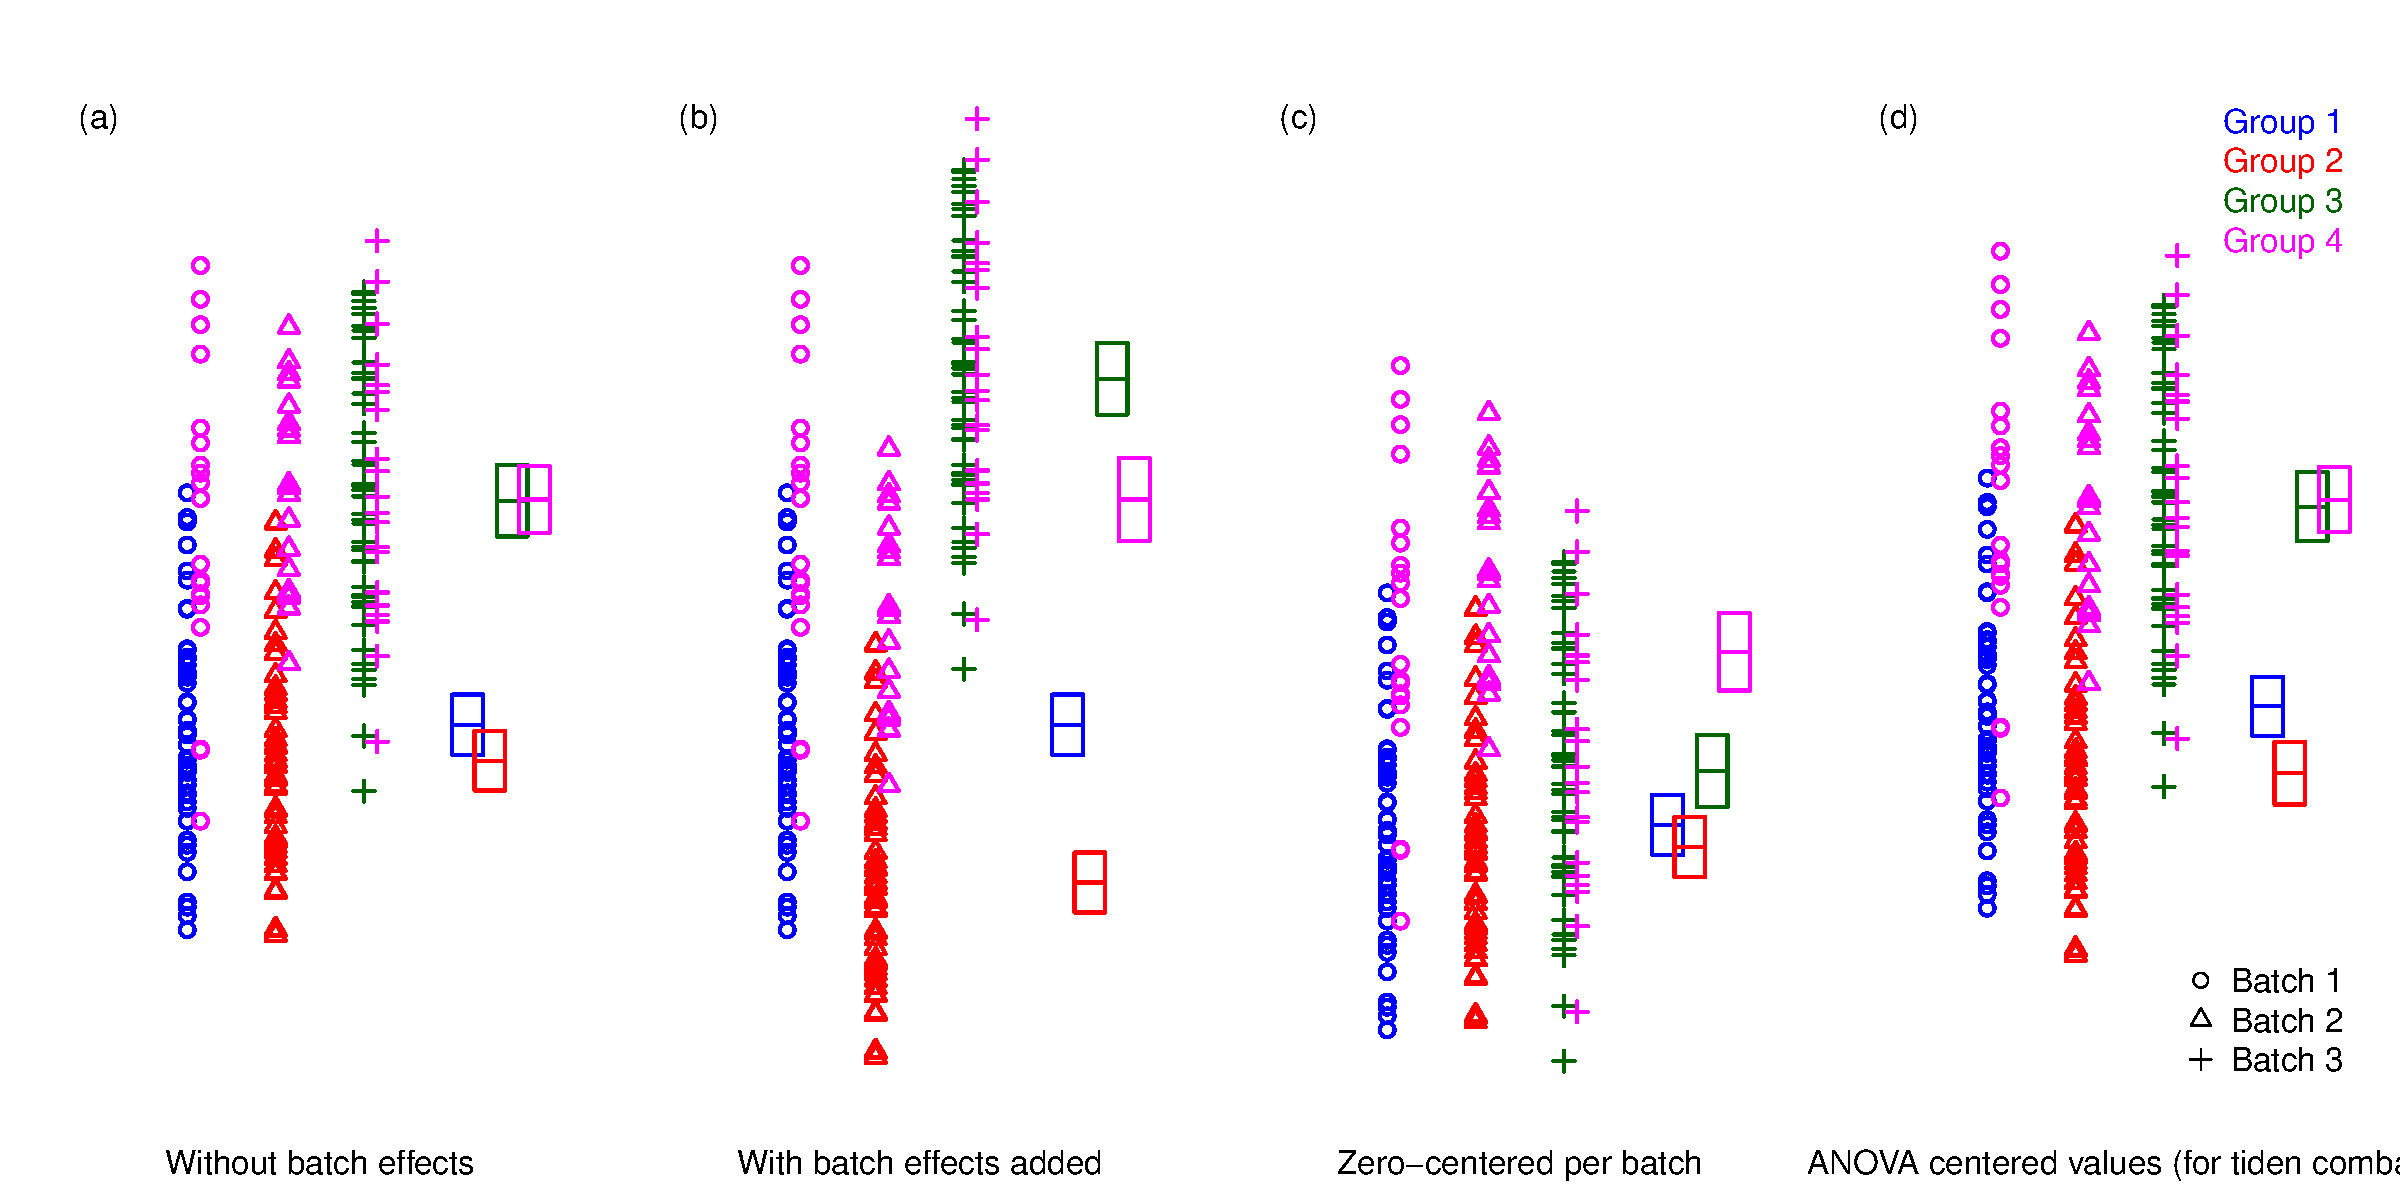
\includegraphics[width=13cm]{Fig/boxplots.pdf}
%\centering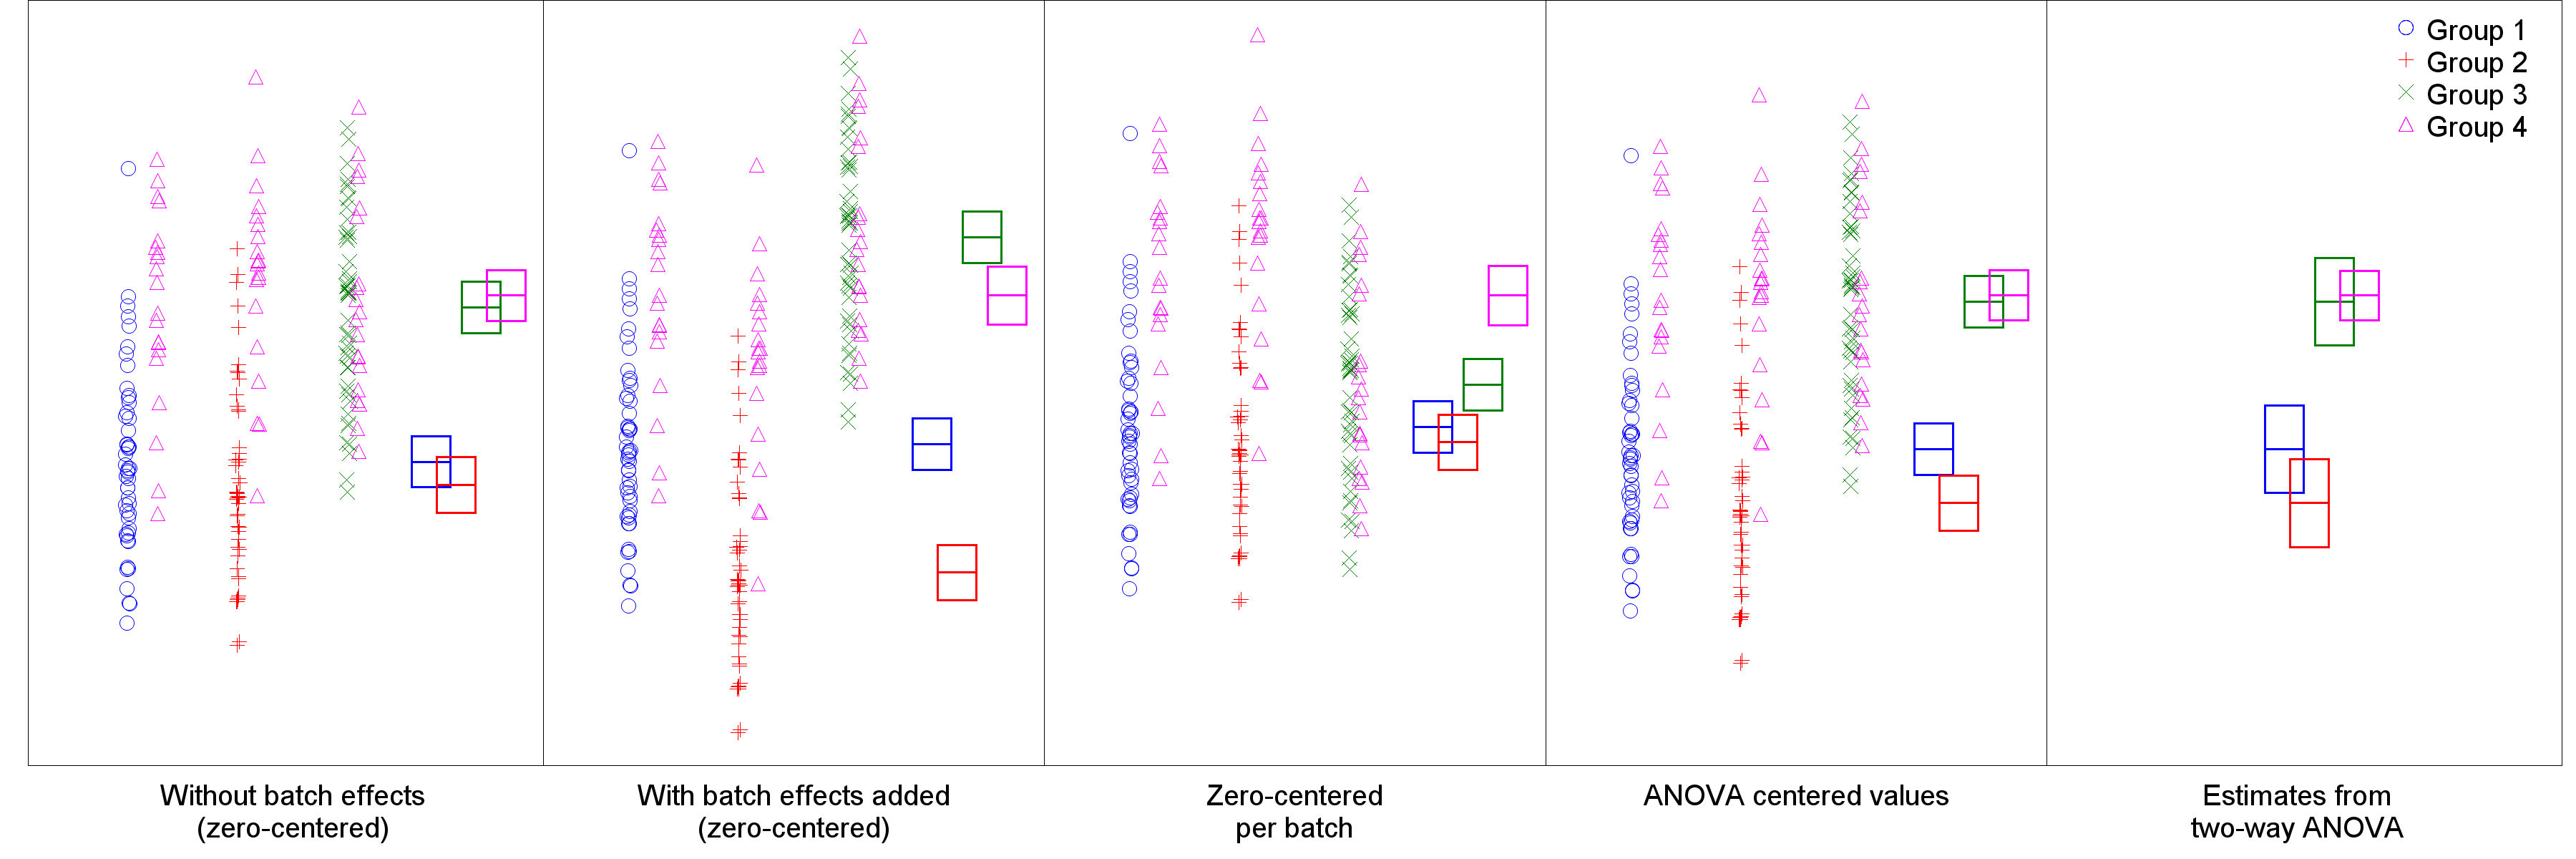
\includegraphics[width=13cm]{Fig/boxplots.png}
\caption{Simulated data from four study groups was generated where groups 1 and 2 have lower means than groups 3 and 4. These were placed in three different batches with batch effects added. Values and boxes showing group mean with 95\%~confidence intervals are displayed for data without batch effects, after adding batch effects, after batch centering, and after two-way ANOVA based batch centering (using \texttt{limma}). The last frame shows the least squares estimates of the group means from a two-way ANOVA. This case, design and effects, was selected to illustrate the spurious effects that may arise.
}
\label{fig:boxplots}
\end{figure}

\begin{figure}[!p]
\begin{center}$
\begin{array}{cc}
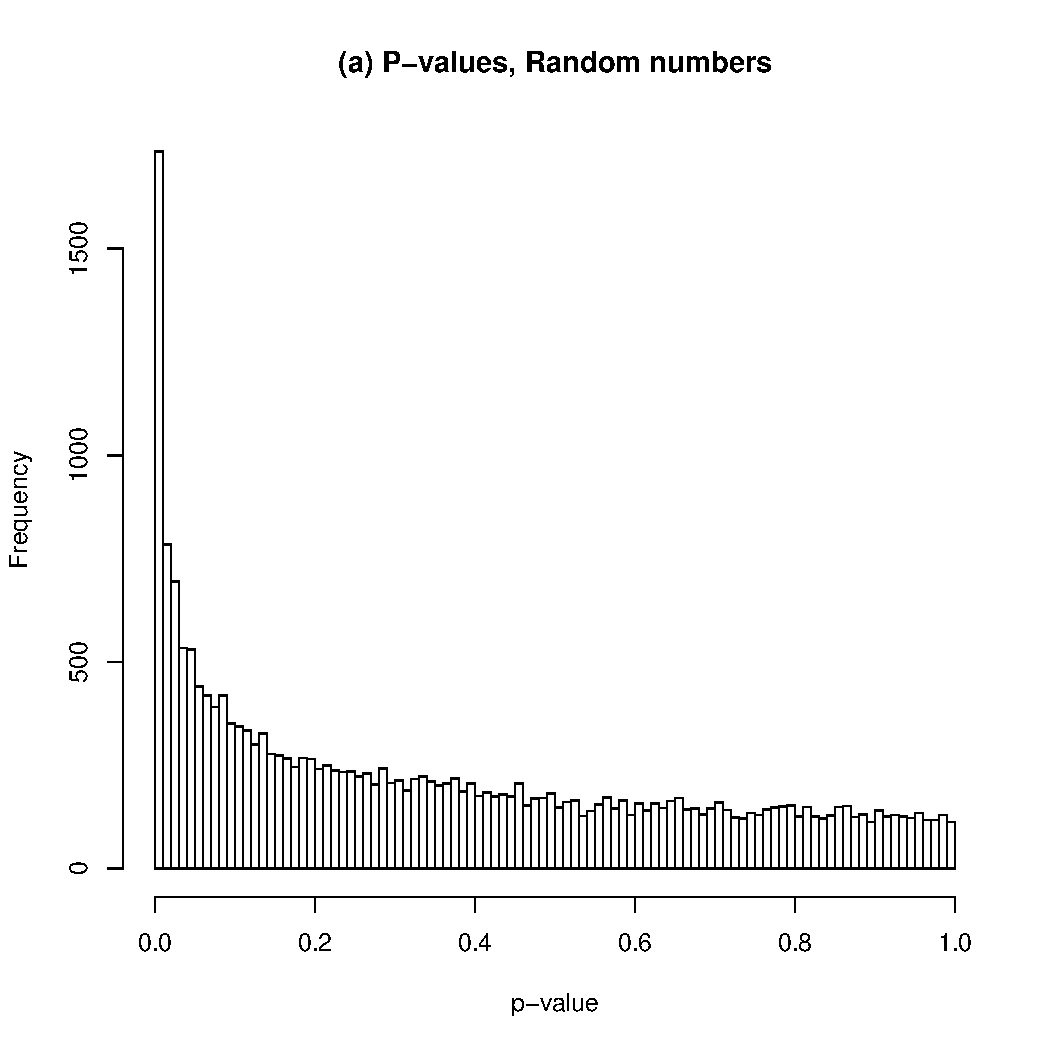
\includegraphics[width=6.5cm]{Fig/leekrandomdatapvalues.pdf} &
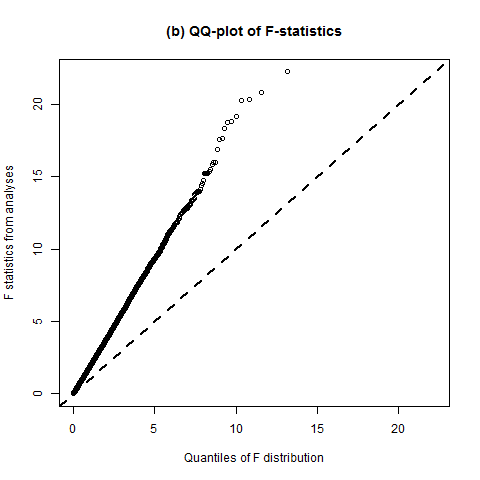
\includegraphics[width=6.5cm]{Fig/leekqqplot.png}
\end{array}$
\end{center}
\caption
{
This is a sanity check where the recommended use of ComBat fails, adapted from the user guide in the \texttt{sva} package. Real data are substituted with random numbers from a normal distribution, but the batch--group design is retained. ComBat is applied followed by an F-test.
a) P-value distribution
b) QQ plot of the F-statistics
}
\label{fig:sanity}
\end{figure}

\begin{figure}[!p]
\begin{center}$
\begin{array}{cc}
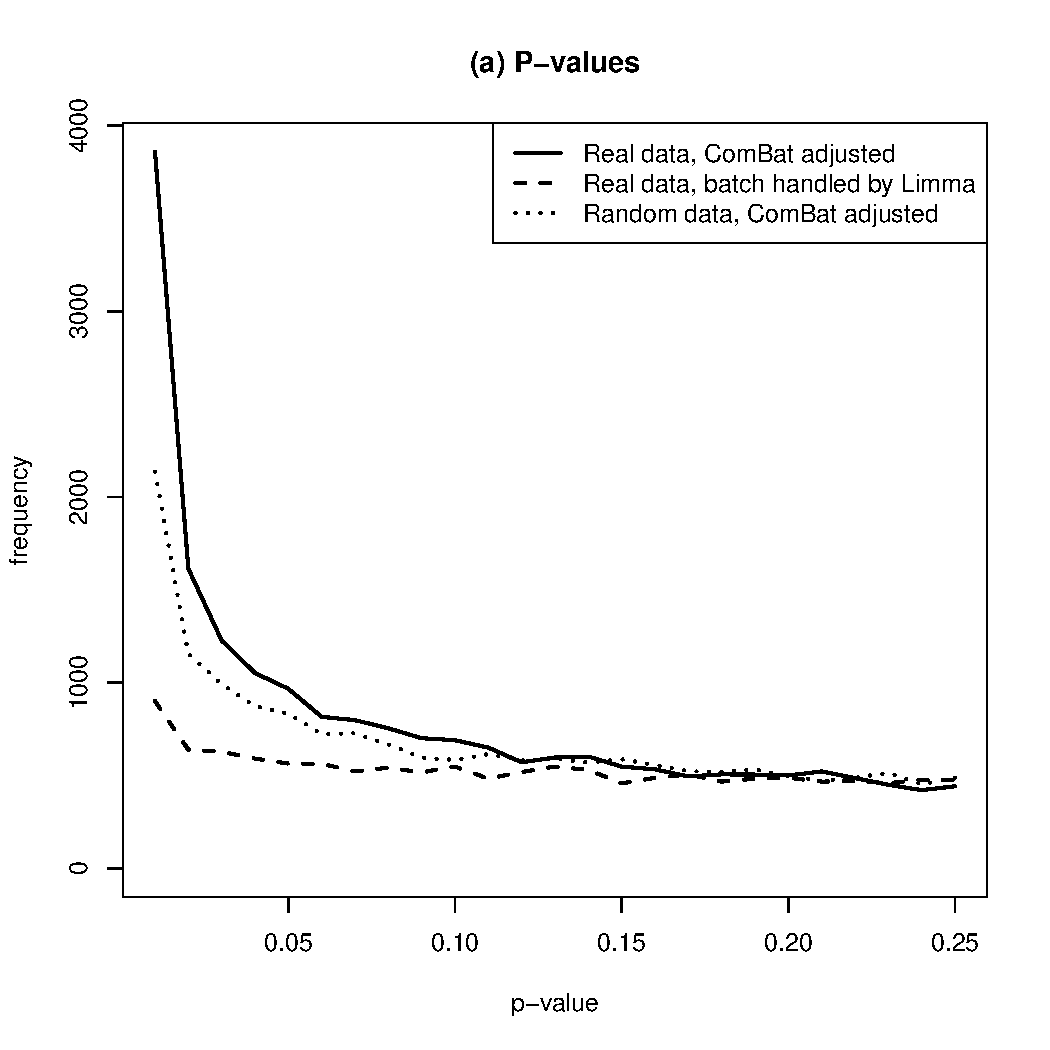
\includegraphics[width=6.5cm]{Fig/towficpvalues.pdf} &
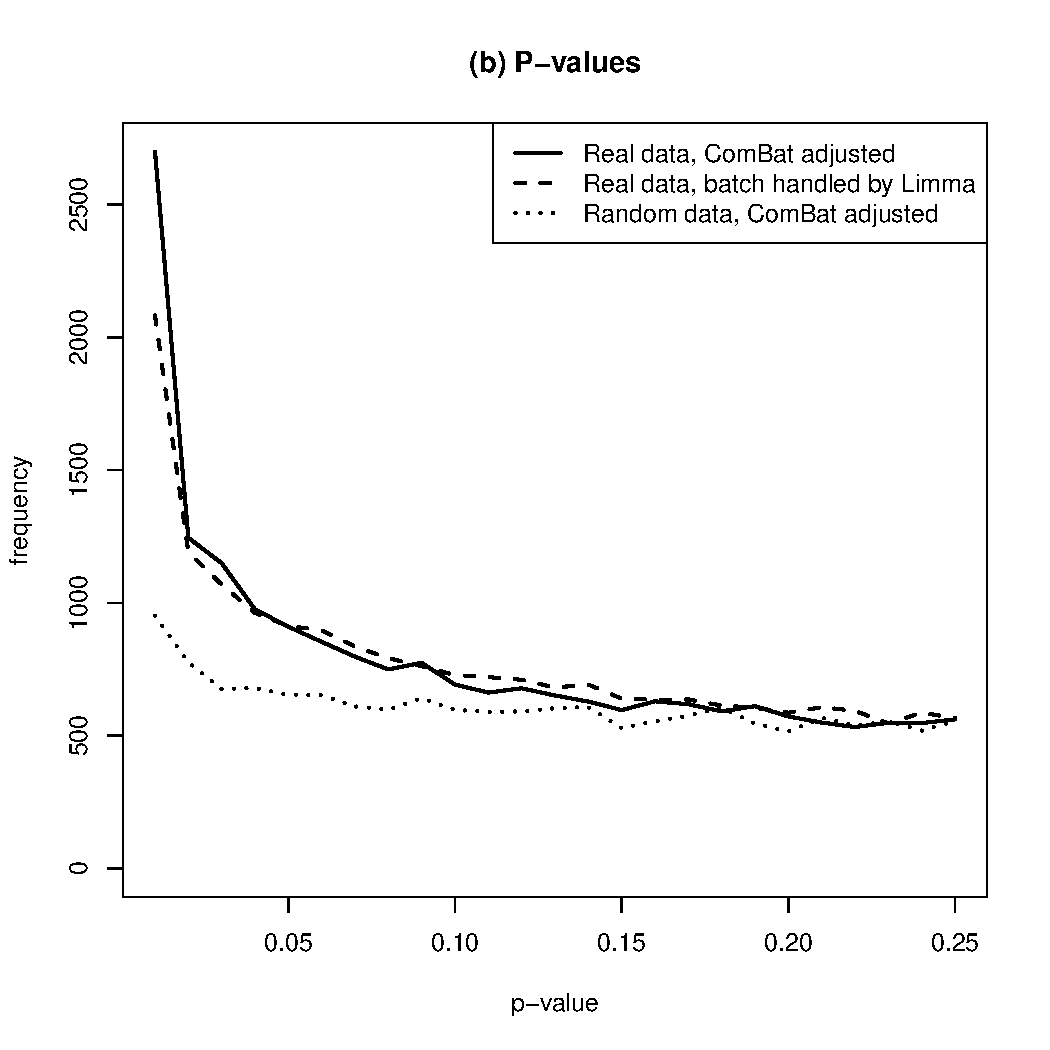
\includegraphics[width=6.5cm]{Fig/johnson2pvalues.pdf}
\end{array}$
\end{center}
\caption
{
Three analyses of two published data sets where batch effects were adjusted for with ComBat. First, analysed as described on the real data using ComBat. Secondly, with ComBat but with random numbers instead of real data. Thirdly, instead of ComBat, analyses of the real data applied \texttt{limma} blocking by batch.
a) Re-analysis of \citet{Towfic2014}, glatiramer acetate vs. generic 
b) Re-analysis of "Data set 2" \citet{Johnson2007},  TAL1 inhibition vs. control
}
\label{fig:comparison}
\end{figure}



\end{document}

